\documentclass{article}
\usepackage[utf8]{inputenc}
\usepackage{graphicx}

\title{Expos\'{e} Master Thesis\\
  Rollup System for Layer 2 Scaling}
\author{Thi Thu Ha Doan \and  Peter Thiemann}
\date{December 2022}

\begin{document}

\maketitle

\section{Design and Implementation of a Prototype for a Rollup System}

% Blockchain systems have grown rapidly in recent years. However, the increased activity has come at
% a cost to the use of the network. Many blockchains have reached their capacity limits. The high
% demand on the network slows down transactions and increases gas prices, so a "scaling solution" is
% needed and becomes an urgent problem. The main goal of scalability is to increase transaction
% speed and throughput while ensuring decentralization and security.  

% Various scaling solutions have been proposed by both industry and academic communities. The
% solutions can be divided into two catalogues: first layer and second layer scaling solutions. The
% first layer scaling solutions (on-chain scaling) require changes to the blockchain protocol. For
% this solution, we can mention Proof-of-stake protocol and Sharding. Second layer scaling
% (off-chain scaling)  uses a separate network called layer 2 (L2) that runs on top of the main
% layer 1 (L1) network and derives the security guarantee from the main network. Current second
% layer scaling solutions include: State Channels, Sidechain, Plasma and Rollup. 

% Rollups are an off-chain scaling solution that reduces computational overhead in the main network
% by moving computation and storage off-chain to L2. Rollup systems inherit the security of the
% mainnet by publishing computation results on the chain, as shown in
% Fig~\ref{rollup-batch}. Rollups process a large number of transactions in a rollup batch and then
% send the compressed summary data defining the changes to the system state to L1. This approach
% allows fixed costs to be spread across multiple transactions in each rollup batch, reducing user
% charges. Rollups therefore provide a significant improvement in transaction throughput. 

% \begin{figure}[t]
% \caption{Rollup systems}
% 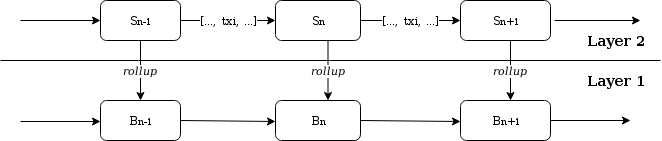
\includegraphics[width=12cm]{rollup-batch}
% \label{rollup-batch}
% \centering
% \end{figure}

The goal of this work is to investigate the design and implementation of a rollup system for the Ethereum blockchain. To make that palatable, we suggest a number of restrictions on the functionality:
\begin{itemize}
\item only transfers of Ether, i.e., there are no contracts on the rollup;
\item optimistic rollup (less ambitious);
\item only a single aggregator (rather than multiple, to avoid the need of a consensus protocol on the roll up).
\end{itemize}

\subsection{Design considerations}
\label{sec:design-consy}

In rollup systems, users sign transactions and submit them to an aggregator (sequencer) that checks, orders, and executes these transactions. The aggregator then compresses the data into a rollup batch and compresses the batch with other necessary data (e.g., system state ) into a rollup block and publishes that rollup block as a single transaction on Layer 1 (L1). There are two different ways to publish the data to the network. The first approach is optimistic rollup, which assumes that the off-chain transactions are valid and does not require validity proofs for the off-chain transactions in the rollup batch. Another approach is zero-knowledge rollup (ZK rollup), in which the aggregator must publish proofs of validity. In contrast, an optimistic rollup responds to a fraud proof to determine where transactions are invalid. After a rollup batch is submitted to L1, anyone can challenge the results of a rollup transaction by computing a fraud proof.

The design should contain only the core components of a rollup system, but it should be designed for extensibility if we want to enrich it for future research. For security, the system relies on a fraud 
detection procedure as in optimistic rollups. A fraud proof is an assertion that a state transition
is invalid and therefore the entire batch should be reversed. The prototype targets the Ethereum
blockchain. Fig~\ref{rollup-design} sketches a possible architecture of the prototype rollup system.

\begin{figure}[t]
\caption{Design of the rollup system}
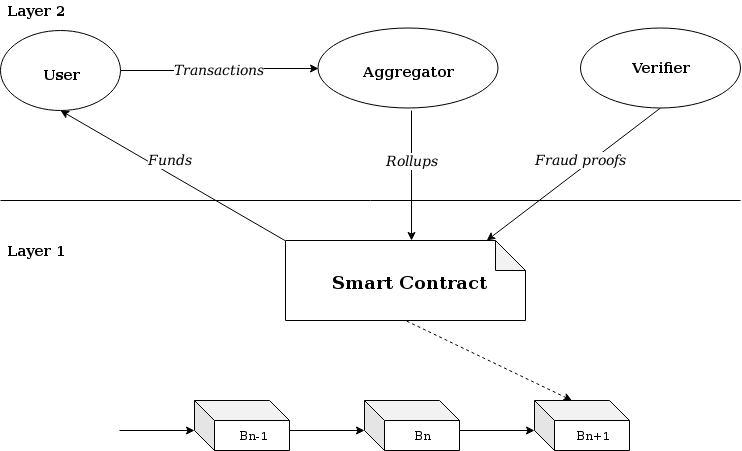
\includegraphics[width=12cm]{rollup-design.png}
\centering
\label{rollup-design}
\end{figure}

\subsection{Interacting with the main network}
As depicted in Fig.~\ref{rollup-design}, the main actors of the rollup system are a moderating smart contract on the main chain, an aggregator, and a verifier.

\subsubsection{On-chain smart contract}
The operation of the rollup system is controlled by a smart contract that is deployed on-chain. Users must deposit funds into the smart contract before they can use the rollup. Funds are then locked in the contract and the user receives a corresponding amount of tokens on the rollup system. The smart contract is responsible  for the following tasks.
\begin{itemize} 
\item registering and deregistering users on the rollup;
\item receiving and processing rollup block summaries; 
\item storing and updating the status of the rollup system;  
\item processing disputes when a verifier submits a fraud proof in the challenge period.
\end{itemize}

\subsubsection{Aggregator}
In a rollup system, a transaction can come from a user in layer 2 (L2) via a direct peer-to-peer network or from L1 via an intermediate contract running on L1. However, in this prototype rollup system, for simplicity, only transactions submitted by and originating from users in L2 are offered. The aggregator receives transactions signed and sent by users. After that, the aggregator
\begin{itemize} 
\item verifies, orders, and executes these transactions off-chain on L2; 
\item bundles the transactions in a rollup batch, forms and publishes a rollup block to L1. 
\end{itemize}
%verifies, orders, and executes them. The aggregator then bundles the off-chain transactions into a rollup batch and sends it to L1 via the smart contract call. In this process, the transaction data is compressed and published on-chain as call data. The published data contains the system state root and the transaction stack in a rollup block in a highly compressed form. Since the calldata is on-chain as part of the history logs, but not stored in the smart contract, it is less expensive.

%A system state constructed as shown in  Fig~\ref{rollup-batch-data} is a term that refers to the available information about the rollup system at a given time. The state includes key information about the network such as accounts, balances, etc. It is organized as a Merkle tree and the root of this tree is the state root, which refers to the last state of the rollup system. Each state transition in the chain results in a new rollup state, which the aggregator determines by computing a new state root. This root state is hashed, sent, and stored in the on-chain smart contract. The aggregator must transmit both the previous and new state roots when it publishes the rollup batches. If the previous state root matches the existing state root in the smart contract, the latter is discarded and replaced with the new state root (post state root).

\subsubsection{Verifier}
The system allows the aggregator to publish rollup batches without providing proof of validity. However, to prevent any misbehaviour by the aggregator, the rollup system proposes a period of time, called the challenge period, during which a verifier can challenge a state transition. When rollup batches are published on L1, the aggregator must deposit a certain amount of funds that is locked until the end of the challenge period. Similarly, the verifier must lock the same amount as the aggregator when disputing the aggregator.

When a verifier initiates the challenge process by submitting a fraud proof, the transactions in the rollup batch are re-executed on-chain to determine who wins the challenge. If the aggregator is penalised, as a result, half of the aggregator's deposit is transferred to the verifier and the other half is burned. If the verifier fails to prove the aggregator's wrongdoing, the same will happen with the verifier's deposit.

A verifier is responsible for
\begin{itemize} 
\item watching the rollup system to detect a published batch with invalid transactions and turn it into a fraud proof;
\item starting the dispute process by submitting a fraud proof to L1 when it finds an invalid batch; 
\item cooperating with L1 in the dispute process.
\end{itemize}

\subsection{Data availability}
Since a malicious aggregator can steal funds by publishing invalid transactions, the security of the system relies on honest verifier(s) re-executing transactions in a rollup batch and submitting a fraud proof to challenge invalid state transitions. Since on-chain execution is based on the published data, the data availability is critical because without access to this data, the verifier cannot create fraud evidence. The data contains the transaction batch and other necessary data in a rollup block in a highly compressed form and is published on-chain as calldata for the smart contract.
%A system state is a term that refers to the available information about the rollup system at a given time. 
%The state includes key information about the network such as accounts, balances, etc.

Publishing the full transaction data on the mainnet could be expensive. Therefore, the rollup system uses compression techniques to reduce the amount of transaction-related data. Compression of the data is achieved by publishing only the information required to deterministically re-execute the transaction.

%\begin{figure}[t]
%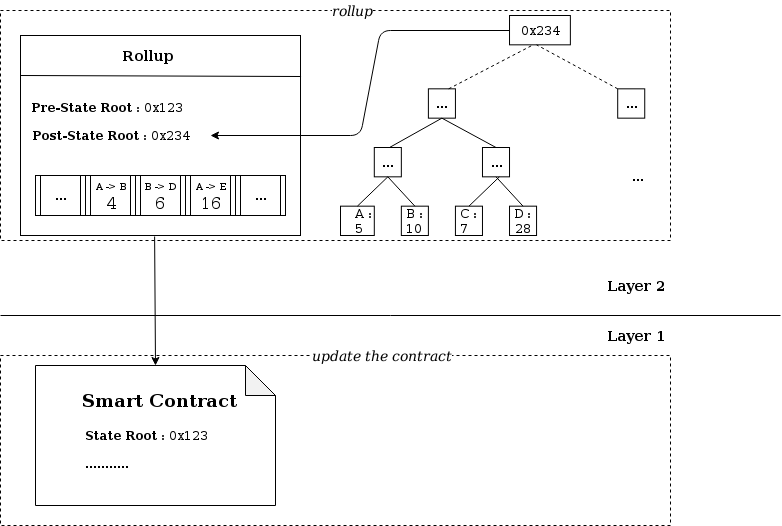
\includegraphics[width=12cm]{rollup-batch-data}
%\centering
%\label{rollup-batch-data}
%\end{figure}
%\subsection{Dispute period}
%The system allows the aggregator to publish rollup batches without providing proof of validity. However, to prevent any misbehaviour by the aggregator, the rollup system proposes a period of time, called the challenge period, during which anyone can challenge a state transition. This actor is called a verifier in our model. Note that when rollup batches are published on L1, the aggregator must deposit a certain amount of funds that is locked until the end of the challenge period. Similarly, the verifier must lock the same amount as the aggregator if it wishes to challenge the aggregator.

%When a verifier initiates the dispute process by submitting a fraud proof claiming that a state transition is invalid and therefore the entire batch should be reversed, the system reruns the transactions in the rollup batch on the master chain to calculate the post-root state that determines who wins the challenge. If this root state is different from the one specified by the aggregator, the aggregator is penalised. As a result, half of the aggregator's deposit is transferred to the verifier and the other half is burned. If the verifier  fails to prove the aggregator's misconduct, the same will happen to the verifier's deposit.

\section{Tasks}
\subsection{Related work: Survey of current rollup technologies}
\begin{itemize} 
\item Optimistic rollups. 
\item ZK rollups. 
\item The efficiency of rollups for Layer 2 scaling.
\end{itemize}
\subsection{Exploration of technologies}
\begin{itemize} 
\item The state tree and state root. 
\item Data compression: various techniques for compressing transaction data. 
\item Dispute progress.
\end{itemize}
\subsection{Development of rollup system}
\begin{itemize} 
\item Design, code, and deploy the smart contract on the chain. 
\item Design and implement L2 system. 
\item Develop the interface for interaction between L1 and L2.
\end{itemize}
\end{document}
